\documentclass[12pt]{article}

% for special characters
\usepackage[utf8]{inputenc}
% for images
\usepackage{graphicx}
\graphicspath{{img/}}
% for source in images
\usepackage{floatrow}
% for urls
\usepackage{url}
% for references
\usepackage[sorting=none]{biblatex}
\addbibresource{references.bib}
% for multiple images
\usepackage{subfig}
% for automatic reference prefix
\usepackage{hyperref}

\begin{document}

\title{
\vspace{-2.0cm}

\includegraphics{zhaw}\\ 
\vspace{3cm}
Deep learning classification of rheumatoid arthritis\\
{\Large Zurich University of Applied Sciences}}
\author{\begin{tabular}{rl}
  \textbf{Author:} & Janick Rohrbach \\
  \textbf{Supervisor:} & Dr. Oliver Dürr \\ & Prof. Dr. Beate Sick \\
  \textbf{Industrial Partner:} & Seantis GmbH \\
  \textbf{External Supervisor:} & Fabian Reinhard \\ & Dr. Tobias Reinhard \\
  \textbf{Date:} & December 12, 2017 \\
  \hspace{6.0cm} & \hspace{6.0cm}
\end{tabular}}
\date{}
\maketitle

\newpage

\section*{Declaration of originality\\ \large{Project Thesis at the School of Engineering}}
By submitting this project thesis, the undersigned student confirms that this thesis is his own work and was written without the help of a third party. \\
\\
The student declares that all sources in the text (including Internet pages) and appendices have been correctly disclosed. This means that there has been no plagiarism, i.e. no sections of the project thesis have been partially or wholly taken from other texts and represented as the student’s own work or included without being correctly referenced. \\
\\
Any misconduct will be dealt with according to paragraphs 39 and 40 of the General Academic Regulations for Bachelor’s and Master’s Degree courses at the Zurich University of Applied Sciences (Rahmenprüfungsordnung ZHAW (RPO)) and subject to the provisions for disciplinary action stipulated in the University regulations.\\
\vspace{3cm} \\
City, Date: \hspace{5cm} Signature:

\newpage

\section*{Abstract}
Abstract goes here

\newpage

\section*{Acknowledgements}
I would like to express my sincere thanks to my supervisors Beate Sick and Oliver Dürr who provided me with guidance and support during the writing of this thesis. 

I would also like to thank Fabian Reinhard and Tobias Reinhard (Seantis GmbH) for their valuable inputs. 

Further, I want to acknowledge the SCQM foundation which made this thesis possible through their immense dataset. A list of rheumatology offices and hospitals that are contributing to the SCQM registries can be found on www.scqm.ch/institutions. The SCQM is financially supported by pharmaceutical industries and donors. A list of financial supporters can be found on www.scqm.ch/sponsors.

\newpage

\tableofcontents

\newpage

\section{Introduction}

This thesis shows a method for the automated scoring of x-ray images of patients with rheumatoid arthritis. 

\subsection{Background}

Rheumatoid arthritis is caused by a malfunctioning immune system. It is therefore a type of autoimmune diseases. The immune system attacks healthy tissue instead of bacteria and viruses. This causes inflammation in the joints. Irreversible damage to the bone in the joint can occur, if the inflammation lasts for a long time. \cite{rheuma} Rheumatoid arthritis is incurable, merely the symptoms can be treated.

Today, the severity of the bone erosion is assessed by a trained rheumatologist by using x-ray images of hand and feet. This process takes several minutes per patient. Recent advances in computer vision make it possible to automate this task. This leads to time savings which in return helps the rheumatologist to spend more time with the patient.

The Swiss Clinical Quality Management in Rheumatic Diseases (SCQM) Foundation runs a national registry of inflammatory rheumatic diseases. \cite{scqm_about} They have collected anonymized patient data for over 10 years and provide us with x-ray images for this analysis.

Seantis GmbH is a Swiss company that develops data driven web applications for medical research, pubic administration and aviation. \cite{seantis_about} For their customer SCQM they want to automate the bone erosion assessment. They already have a working algorithm, which detects the body part shown in the x-ray image. A second algorithm detects the joints in the image and extracts them as single images. These images are then used together with the bone erosion scores to train our model.

% Stand der Technik: Bisherige Lösungen des Problems und deren Grenzen 
% (Nennt kurz den Industriepartner und/oder weitere Kooperationspartner und dessen/deren Interesse am Thema Fragestellung) 

\subsection{Related literature}

% Nennt bestehende Arbeiten/Literatur zum Thema Literaturrecherche

There are several applications where convolutional neural networks are used in medical research.

A recent paper from Tajbakhsh et al. \cite{tajbakhsh_2017} investigated whether fine-tuning a pre-trained CNN is better than training a CNN from scratch when applied to medical images. They find that pre-trained networks with fine-tuning always outperformed or at least performed as well as CNNs trained from scratch. They further recommend a layer-wise fine tuning which seems to outperform shallow and deep tuning.

A study by Paul et al. \cite{paul_2017} tried to classify osteoporosis by considering x-ray images of the bone. This task proved to be very difficult as the x-ray images from healthy patients look very similar to the ones of patients with the disease. By using a transfer learning approach they achieved a validation accuracy of 44.82 \%.

Zhou et al. \cite{zhou_2002} used a two-level ensemble of neural networks to identify lung cancer cells on x-ray images of the chest. The first-level ensemble classifies whether a cell is a cancer cell or not by using full voting. The second-level ensemble is used only on cells classified by the first-level as cancer cells. It differentiates between different cancer classes as well as a non-cancer class. This ensemble works with plurality voting. The authors state that this method achieves a high accuracy and a low rate of false negatives.

A report from Chen \cite{chen_2016} showed the application of convolutional neural networks on x-ray images of hands to predict the developmental bone age. He achieves a top one and two accuracy of 46 \% and 70 \% respectively. This result is close to previously used methods which use manual segmentation and handcrafted features.



% Kaggle Diabetic Retinopathy Detection



\subsection{Aim and scope of this thesis}

The aim of this thesis is to predict bone erosion scores from x-ray images. We further examine how the bone erosion and the disease activity are correlated and use a time series of images to predict the course of the disease.

The work is based on images of the left hand only. There exist also images of right hands as well as left and right feet. But at this point in time, only the joints of left hands have been extracted from the images. We assume that the model will perform similar on the joints of the right hand. By fine-tuning the model on the images of joints from feet it should also perform well for those images.


% Formuliert das Ziel der Arbeit
% Verweist auf die offizielle Aufgabenstellung des/der Dozierenden im Anhang

\subsection{Outline}

\autoref{sec:theory} provides...

\noindent\autoref{sec:methods} describes..

% (Übersicht über die Arbeit: stellt die folgenden Teile der Arbeit kurz vor)


\newpage

\section{Theory}
\label{sec:theory}

\subsection{Bone erosion scores}
\label{subsec:bone_erosion}

\autoref{fig:joints} shows a sample x-ray image of two hands similar to the images received from the SCQM foundation. The five proximal interphalangeal (PIP) joints and the 5 carpometacarpal (MCP) joints per hand are shown with blue bounding boxes. A trained rheumatologist has scored each of those 10 joints per hand.

\begin{figure}[ht]
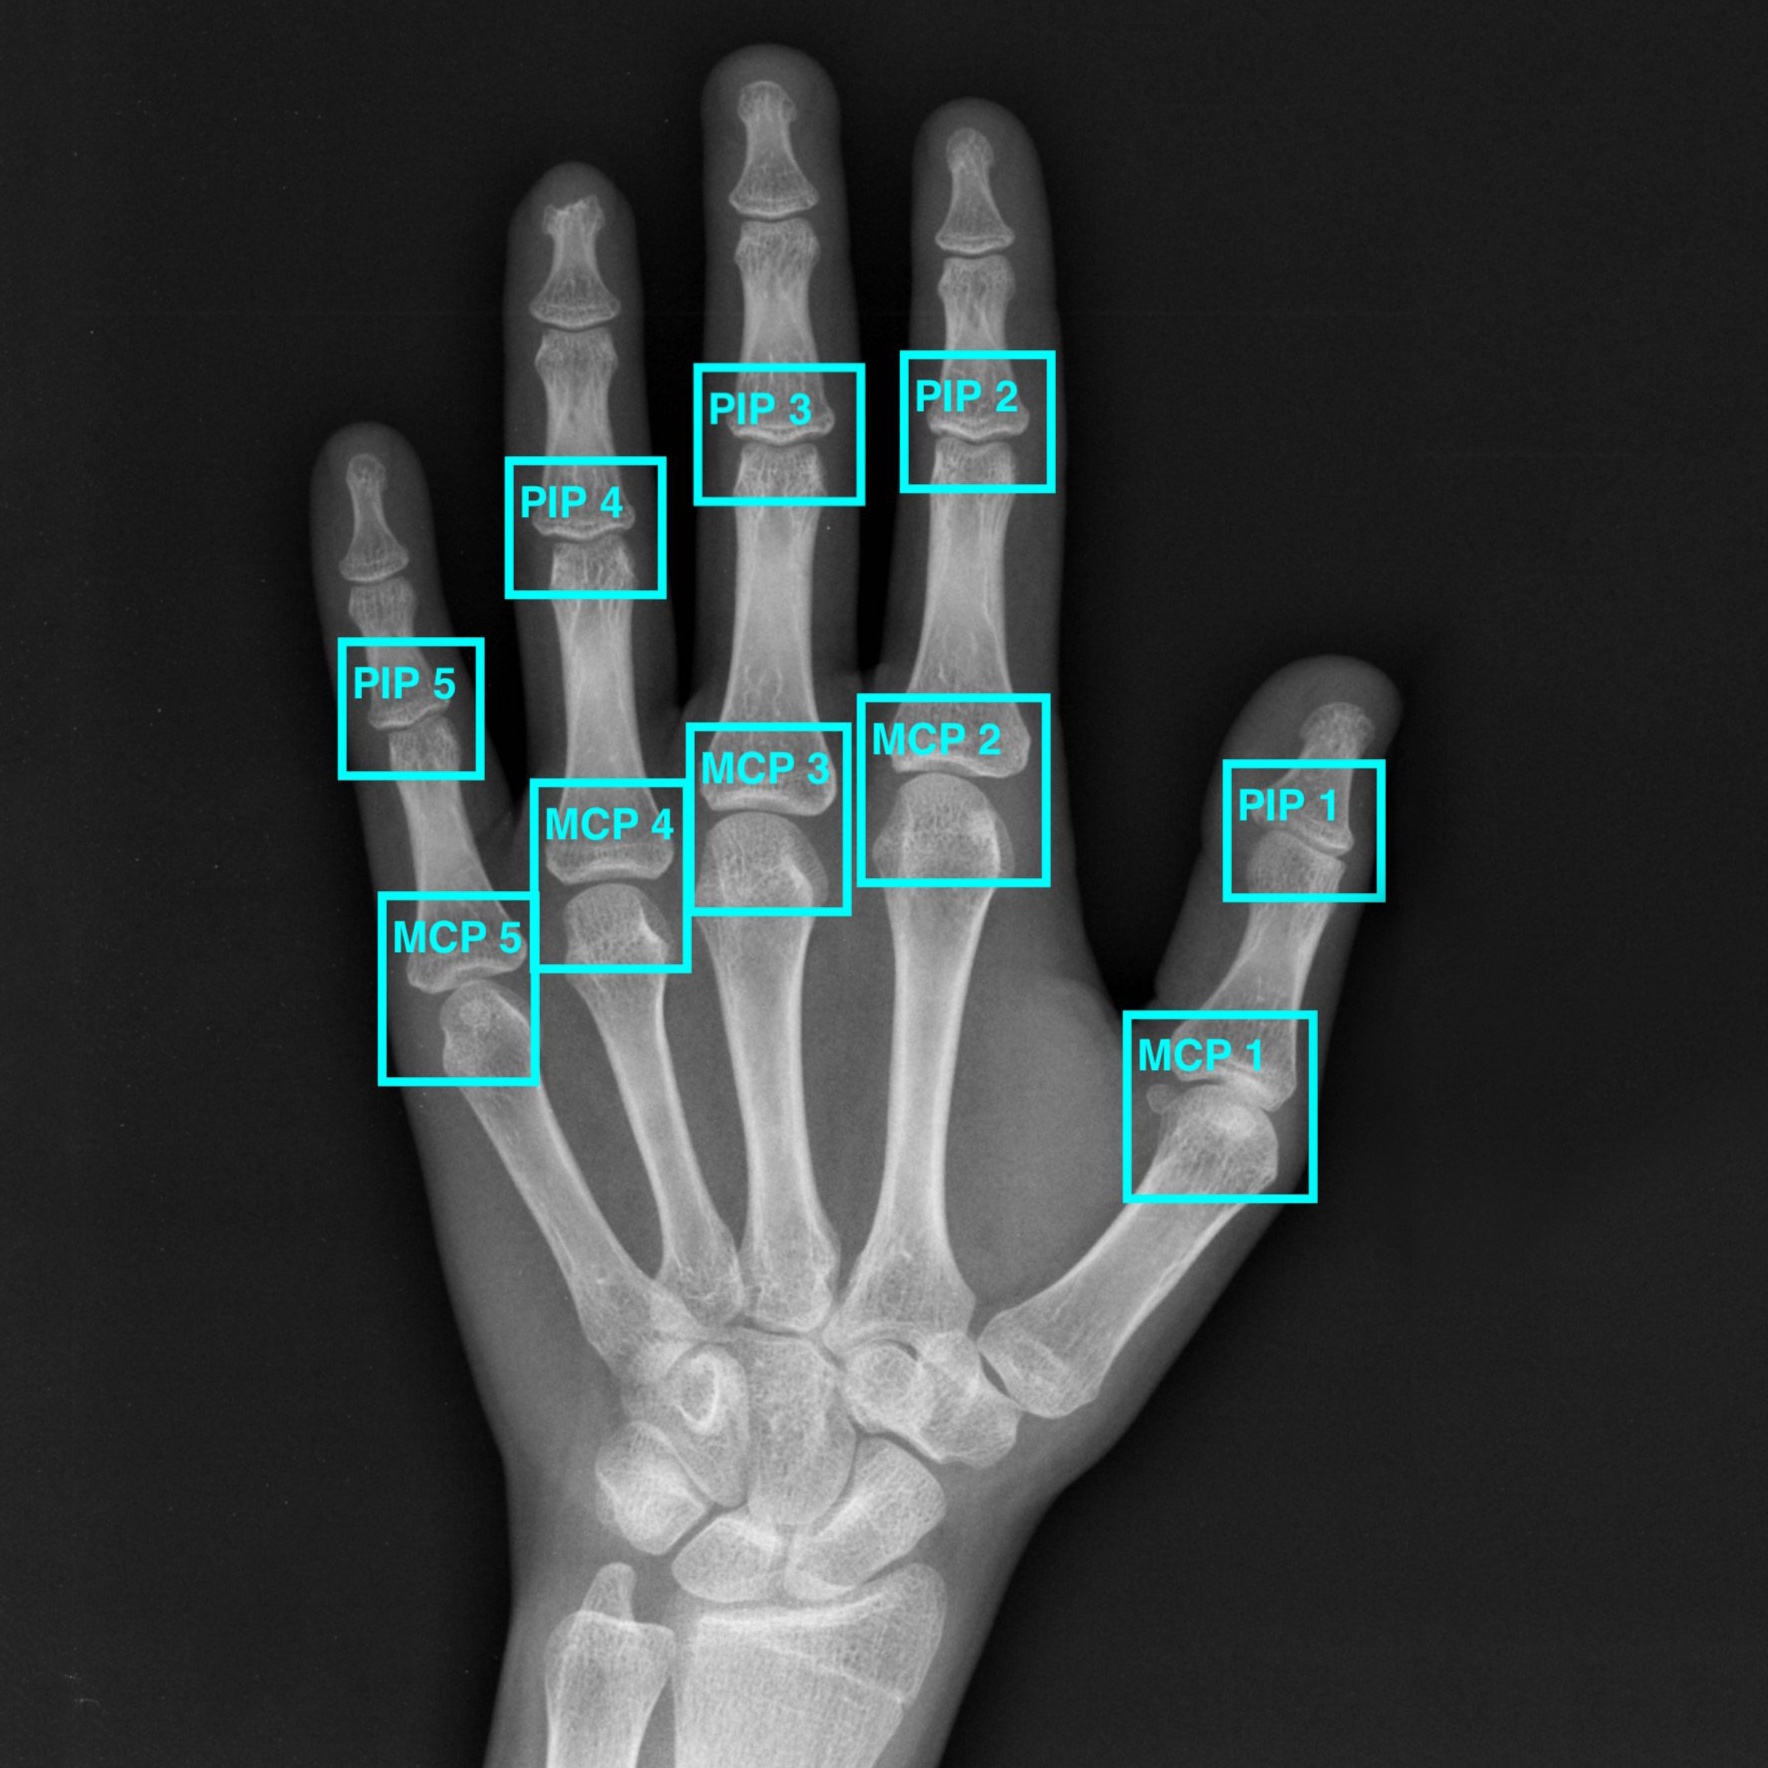
\includegraphics[width=10cm]{joints}	
\caption{Proximal interphalangeal (PIP) joints and carpometacarpal  (MCP) joints.}
\floatfoot{Original image by Nevit Dilmen (CC BY-SA) \url{https://commons.wikimedia.org/wiki/File:Medical\_X\-Ray\_imaging\_OPC06\_nevit.jpg}}
\label{fig:joints}
\end{figure}


\subsubsection{Ratingen score}
\label{subsubsec:ratingen}

% hier fehlt noch quelle für tabelle plus text dazu. DOI
%https://doi.org/10.1007/978-3-7985-1721-9_2
 %Publisher Name
%Steinkopff
 %Print ISBN
%978-3-7985-1720-2
%Online ISBN
%978-3-7985-1721-9

\begin{tabular}{ l c l }
  Stadium 0 & = & normal joint \\
  Stadium 1 & = & one or more erosions, less than 20 \% of the joint surface is eroded \\
  Stadium 2 & = & 21 \% - 40 \% of the joint surface is eroded \\
  Stadium 3 & = & 41 \% - 60 \% of the joint surface is eroded \\
  Stadium 4 & = & 61 \% - 80 \% of the joint surface is eroded \\
  Stadium 5 & = & more than 80 \% of the joint surface is eroded \\
\end{tabular}




\subsection{Convolutional neural networks}
\label{subsec:cnn}
Convolutional neural networks take an image as an input. The image then gets passed through several convolutional layers. These layers work as filters and detect different features in the image. The weights of these layers are combined to class scores. Andrey Karpathy provides a good overview over convolutional neural networks in his course notes for the Stanford class CS231n. \cite{cnn}



\section{Methods}
\label{sec:methods}


\section{Predicting Rau scores}

\subsection{Pre-processing}

The pre-processing step formats the images into a suitable format that can be used as an input for the CNN. 

The images of the joints have varying exposure. Some images are very dark while others are very bright. It was therefore considered to apply a histogram equalization, which is a linear transformation that maps the lightest pixel to 255 and the darkest pixel to 1. However, this transformation did not improve the accuracy of the model and was not used for the final model.

\begin{figure}[ht]
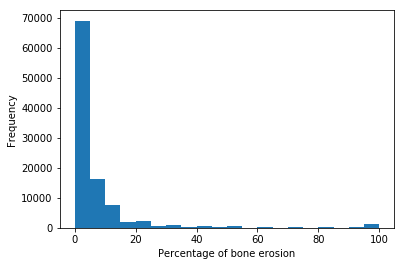
\includegraphics[width=10cm]{imbalance}	
\caption{Distribution of the Rau scores}
\label{fig:imbalance}
\end{figure}

The Rau scores of the labeled joints are highly imbalanced. As seen in \autoref{fig:imbalance} most of the joints are healthy and received a score of 0. There are quite a few observations with scores between 0 and 25 but there are very little observations with scores higher than 25. Because the CNN minimizes the overall loss-function, it would perform bad for the underrepresented part of the data. In this case, the model would be bad in predicting high scores. In order to make the model a good predictor for all cases, we introduced ...????????????







% varying exposure

% imbalanced data

\section{Results}


\section{Discussion}


\section{Conclusion}



\newpage
\printbibliography

\newpage
\listoffigures


\end{document}
